\subsection{Kraft, Arbeit, Leistung}
    \subsubsection{Kraft im el. Feld}
        \mathbox{\overrightarrow{F_E} = Q \overrightarrow{E_0}}
    
    \subsubsection{Arbeit im el. Feld}
        Die gespeicherte Energie ist jeweils die verrichtete Arbeit: $\Delta E = W$
        Arbeit $=$ Kraft $\cdot$ Weg
        \begin{empheq}[box = \fbox]{align*}
            W &= \int \overrightarrow{F}d\overrightarrow{s} = Q \Delta \Phi\\
            &= QU = U \cdot I \cdot t\\
            dW &= UI dt
        \end{empheq}
        \begin{center} \underline{\textbf{Gespeicherte Energie im Kondensator:}} \end{center}
        \begin{minipage}{0.49\linewidth}
            \begin{itemize}
                \item Energie entspricht Fläche unter Q-U-Diagramm.
                \item Ladevorgang eines Kondensators verläuft linear.
                \item Somit: Energie entspricht Dreiecksfläche mit Seitenlänge Ladung und Spannung nach Ladevorgang.
            \end{itemize}
        \end{minipage}
        \begin{minipage}{0.49\linewidth}
            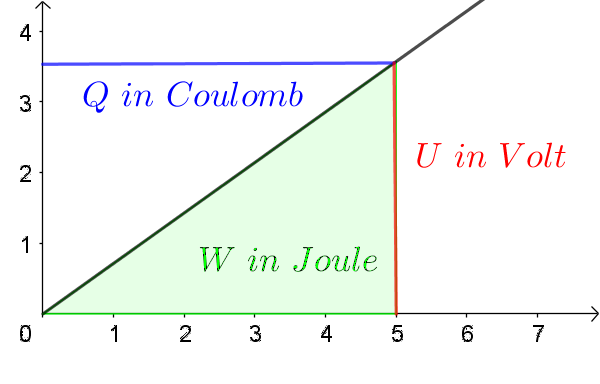
\includegraphics[width = 1\linewidth]{src/images/ladevorgang_kondensator.png}
        \end{minipage}

        \begin{minipage}{0.69\linewidth}
            \begin{empheq}[box = \fbox]{align*}
                W &= \int U dq = \frac{Q U}{2} =  \frac{Q^2}{2C} = \frac{CU^2}{2}\\
                &= \frac{1}{2} \varepsilon_0 E_0^2 V\\
                \rho_{el} &= \frac{W}{V} = \frac{1}{2} \varepsilon_0 E_0^2
            \end{empheq}
        \end{minipage}
        \begin{minipage}{0.29\linewidth}
            \begin{scriptsize}
                \begin{empheq}{align*}
                    Q = &\text{Ladung}\\
                    U = &\text{Spannung}\\
                    C = &\text{Kapazität}\\
                    E_0 = &\text{Elektrische Feldstärke}\\
                    V = &\text{Volumen zwischen}\\
                    &\text{Kondensatorflächen}\\
                    \rho_{el} = &\text{Energiedichte}
                \end{empheq}
            \end{scriptsize}
        \end{minipage}

    \subsubsection{Leistung im el. Feld}
        \mathbox{P = \frac{W}{t} = \frac{F}{v} = U \cdot I}
    